\section{Review of the Published Literature}
This literature review explores a variety of studies revolving around LoRaWAN and focuses on the fundamental end device setup, signal strength measurement, IoT cloud architecture and inherent limitations of the technology. LoRaWAN has gained traction for its promise of long-range, low-power solutions to WSNs which is critical for IoT applications. However, there are significant research gaps in the literature regarding the reliability and concistency of LoRaWAN in various environmental conditions and its practicality for applications requiring real time response. This review aims to evaluate these research gaps and evidence the design and optimization considerations for the LoRaWAN-based Structural Health Monitoring (SHM) deployment for the Griffith footbridge. The literature synthesized in this review is instrumental in shaping the approach and methodology of this research project. 

One application of LoRaWAN is in the field of Agro-Informatics, as demonstrated by Gehani et al. (2021) \cite{LoRa-Agro-Informatics}. Their research focused on utilizing LoRaWAN IoT architecture for the detection and classification of plant pathogens. The signal strength of the transmitted LoRa packets was evaluated through Received Signal Strength Indicator (RSSI) and Signal-to-Noise Ratio (SNR) at various depths from 0 cm to 60 cm. Their findings suggest that LoRa transmitters can function effectively provided the depth does not exceed 50 cm. A diagram of the experimental setup is shown in figure \ref{lora-bucket}. This research serves as a valuable foundation for designing the enclosure thickness that will be used in this project. 

\begin{figure}[h]
	\centering
	\caption{Experimental Setup for LoRa Node in Soil \cite{LoRa-Agro-Informatics}}
	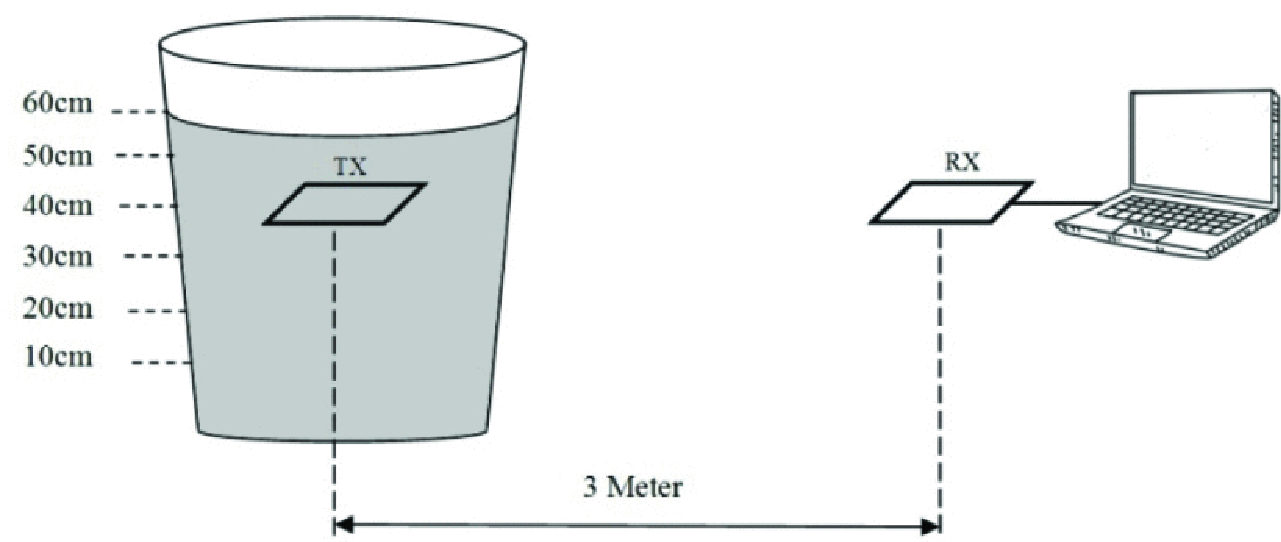
\includegraphics[scale=0.5]{Sections/Literature-Review/Lora-bucket.pdf}
	\label{lora-bucket}
\end{figure}

Fox et al. (2019) \cite{IoT-Regional-Service} expanded on the architecture of LoRaWAN-based IoT systems with a focus on wind turbine monitoring in Ireland. Their study comprised three main components: an end device, a gateway, and an IBM IoT cloud platform. This research demonstrated a comprehensive IoT cloud architecture deployment, covering real-time monitoring, concurrent read/write processes, and database service implementation. Despite the successful deployment, challenges such as LoRa's limited transmission capacity and application specific end device battery life were highlighted, emphasizing the need for future optimization. In terms of practical application, end devices must be optimized to strike a balance between computational load and current draw to achieve sufficient longevity. Figure \ref{Example-GUI} displays an example of a GUI displaying real time data visualization from the Red Node Cloud Foundry application flow within the IBM cloud. The LoRa payload is extracted, processed and displayed in an interface by assigning relative values to their respective interface nodes. With the knowledge gained from this research, the variables from the LoRa payload in this project will be extracted using Arduino IoT cloud variables, and an Arduino IoT cloud dashboard will be used to plot relevant time series data. The Arduino LoRaWAN Adaptive Data Rate (ADR) mechanism will be used in this project to optimise the airtime, data rate and power consumption of the LoRaWAN deployment. This will assist in striking the balance between computational load and current draw of the LoRa node. 

\begin{figure}[h]
	\centering
	\caption{Example of real time data visualization GUI \cite{IoT-Regional-Service}}
	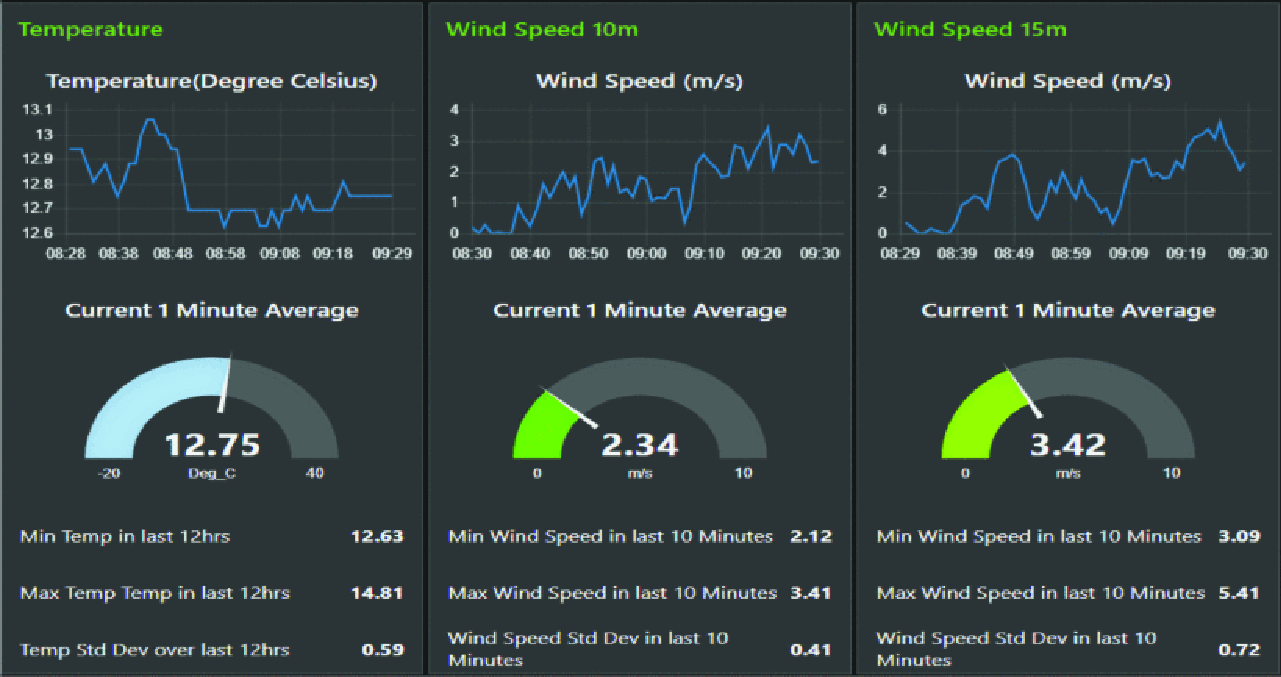
\includegraphics[scale=0.6]{Sections/Literature-Review/Example-GUI.pdf}
	\label{Example-GUI}
\end{figure}

In another exploration of LoRaWAN capabilities, Wildan et al. (2020) \cite{LoRa-Smart-Home} designed and implemented a GUI for smart home systems leveraging LoRa's long-range and low-power benefits. Information such as room temperature is transmitted to a LoRa server through a LoRa client, and is uploaded to a web server. The data is then stored in a database and displayed on a webpage which is accessible from various devices such as a smartphone and laptop. An interface application was created to allow user interaction with the webpage and control over various electronic devices such as lights, TV and air conditioning within the house. The system's performance was tested with a focus on the user experience, web application and delay. This testing was able to address a key limitation in LoRaWAN, the delay in data transmission, noting that while the system performance was generally robust, delays averaged 3.86 seconds. This makes LoRaWAN generally limited for systems that require close to real-time responses. In relation to the smart home, operating the lights and TV with a 3.86 second delay is both significant and noticeable. In its current state this system is functional, but will inevitably invoke hesitancy for mainstream adoption due to an installation cost for a user experience that is not seamless. The delay time evidenced in this study has resulted in avoiding unnecessary downlink messages for this project. This project will only focus on receiving uplink messages with only necessary downlink acknowledgements to avoid the restriction of a delayed response time. 

Maziero et al. (2019) \cite{Monitoring-Electric-Parameters} deployed a real-time monitoring system for tracking electrical quantities at the Federal University of Santa Maria campus. Utilizing Grafana software, they created a panel for tracking both electrical and connectivity metrics, demonstrating the effectiveness of combining LoRaWAN technology and application layer monitoring software for real-time data acquisition and visualization. The study highlights the potential scalability of this system in the sense of feeding data stored in the monitoring center to algorithms capable of autonomously handling the distribution network of electrical metrics, for example automatically altering voltage based on state estimations. It was evident in the research that the ability to monitor electrical quantities in the application layer allowed for the capability of better management and informed decision making based on a holistic interpretation of the distribution network. Figure \ref{Electrical-Monitoring-System} displays the design for the electrical monitoring system and the process of receiving data from The Things Network (TNN) applications and transmitting payloads to a web-based user interface via MQTT and HTTP messaging protocols. The system design of this study gives an excellent context for the chosen implementation of TNN for this project. In this project TNN applications will instead communicate with the Arduino IoT cloud using cloud variables which will be used to plot data on the web-based Arduino cloud dashboard. 

\begin{figure}[h]
	\centering
	\caption{IoT architecture for monitoring electrical quantities \cite{Monitoring-Electric-Parameters}}
	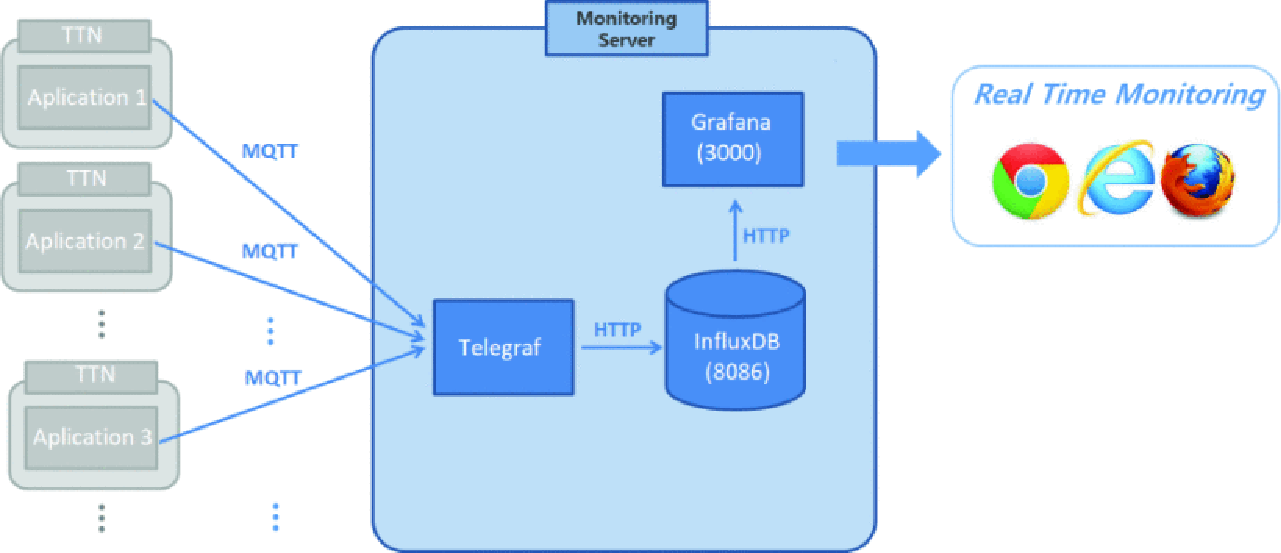
\includegraphics[scale=0.5]{Sections/Literature-Review/Electrical-Monitoring-System.pdf}
	\label{Electrical-Monitoring-System}
\end{figure}

In a study examining the performance of a Smart Gateway network architecture, the authors conducted a series of test focusing on throughput and packet loss \cite{Monitoring-System-Smart-Gateway}. The throughput was found to be inconsistent across a different number of clients where the system was found to have a lower average throughput compared to other LoRaWAN systems due to additional required processing steps. The extra processing steps were attributed to Quality of Service (QoS) parameters, such as measuring packet loss and throughput, processing client data and web server services running on the gateway. The study found a significant packet loss especially when operating with two clients. On average, the system exhibited packet loss of 26\% across a 1-meter range which is a significantly high drop compared to other LoRaWAN implementations. Despite the range limitations, the study concluded that the gateway could support up to 5 clients registering and requesting data automatically, and run LoRa communication alongside the user interface of the information system simultaneously. In light of these findings, this report intends to use the ADR mechanism to automatically optimize QoS since it dynamically chooses the best spreading factor (SF) to send LoRa packets over. Additionally, the gateway used in this project will act as a base station and use the Arduino IoT Cloud and The Things Network (TNN) to handle the network and application layer, removing unnecessary gateway computations. 

Wixted et al. (2016) \cite{LoRa-WSN} conducted reliability testing and discovered a successful connection and acknowledgement request between an end device and gateway across all spreading factors was found to be only 42\% at a distance of 1.9km. After introducing a second gateway this connection rate rose to 70\% and with the introduction of Internet Control Message protocol (ICMP) pings the full connection rate rose to 95.5\%. It was also found that connection was completely lost in isolated stairwells indicating that LoRaWAN is sensitive to obstructions. Thanks to the findings of this research, the deployment of the LoRaWAN system in this project will focus on a short-range setup with minimal obstruction, and focus on the holistic deployment of the IoT architecture. 

In a paper presenting an online test bed for LoRa development, the correlation between packet RSSI and distance was measured \cite{Dandelion-Testbed}. 5 LoRa nodes were placed at distances 500m, 1000m and 1200m away from the gateway, where the nodes placed 100m and 1200m were blocked by urban and natural obstacles. It was found that a low spreading factor (SF) results in a reduction of the packet reception rate (PRR). SF7 was the lowest spreading factor used and was confirmed to only support packet transmission at very low distance. The study concluded that RSSI decreases with distance and that this relationship is directly influenced by the environment, obstacles and spreading factor used for transmission. Various models can be used to model the relationship between RSSI and distance, but as evidenced in figure \ref{rssi-distance-model} the Bor model was closest in predicting correlation. To investigate the RSSI and SNR in this project, the values will be extracted from TNN and plotted over time series. This will further assist in gaining an understanding of the fluctuation of signal strength at a fixed distance from the Griffith footbridge. 

\begin{figure}[h]
	\centering
	\caption{Modelling RSSI-distance correlation. Green represents real data. \cite{Dandelion-Testbed}}
	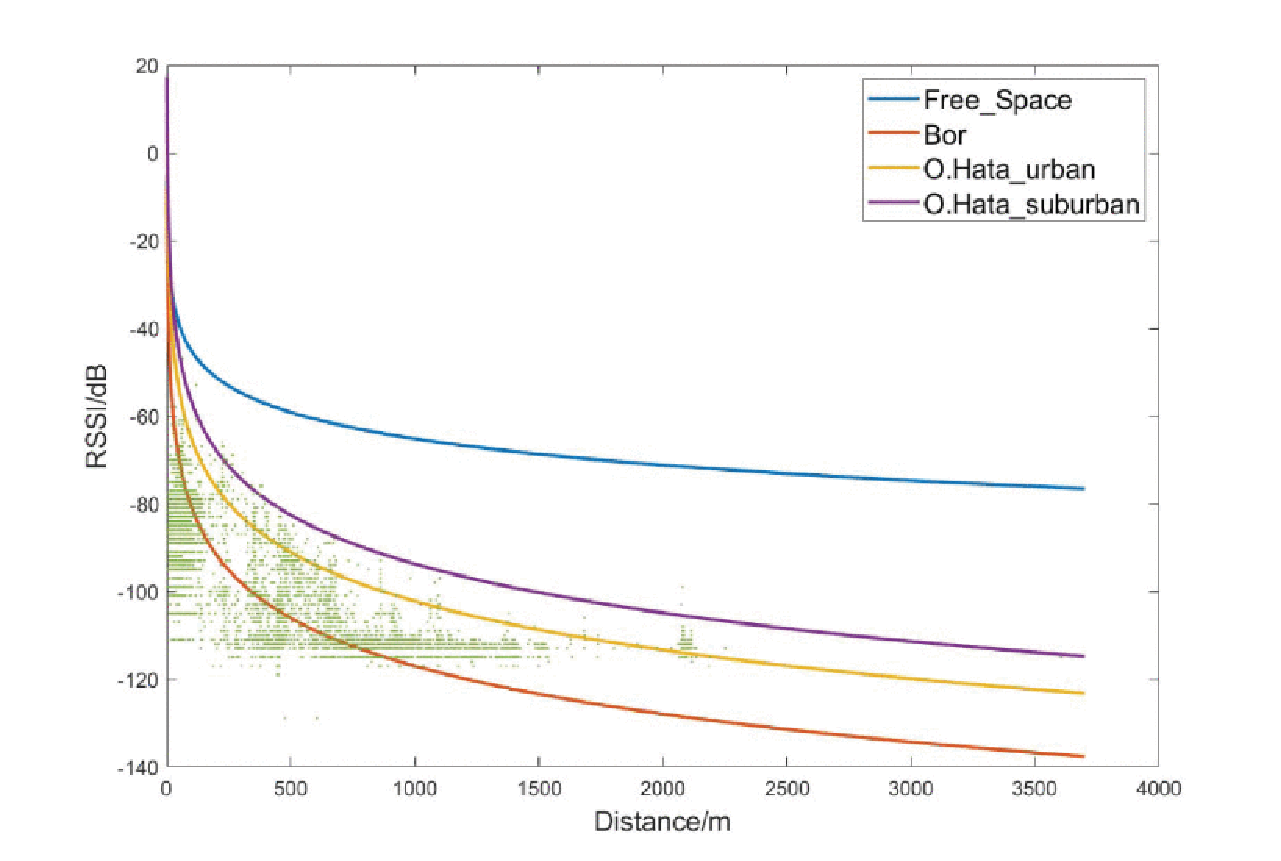
\includegraphics[scale=0.5]{Sections/Literature-Review/rssi-distance-model.pdf}
	\label{rssi-distance-model}
\end{figure}

Jang et al. in 2010 \cite{SHM-Korea} reports the deployment of 70 wireless smart sensor networks (WSSNs) and two base stations on the Jindo Bridge in South Korea. Each sensor facilitates 3-axis acceleration measurement and offers a test bed for structural health monitoring (SHM). Cho et al. in 2010 \cite{WSSN-Korean-Bridge} analysed data collected from these WSSNs, comparing these results to existing acceleration data from a wired monitoring system. The acceleration data collected from the deck and pylons of the bridge revealed a significant acceleration due to vehicle traffic. Vertical and cable vibrations were found to be significant enough for mode extraction and the estimated tension forces for 10 cables were found to lie within a 4\% difference of the previous site inspections using wired monitoring systems. The frequencies of the higher modes were found to exceed those predicted in the finite element (FE) model by less than 16\%, indicating the benefit of WSSN data collection for verifying and amending simulated models. The PSD of the 2007 site inspection using the wired monitoring system is shown in figure \ref{PSD-Wired}. This gives an excellent insight for the expected PSD frequency peaks of the Griffith footbridge, indicating that a maximum peak of approximately 2Hz may appear. 

\begin{figure}[!htb]
	\centering
	\caption{PSD of vertical acceleration with wired monitoring system \cite{WSSN-Korean-Bridge}}
	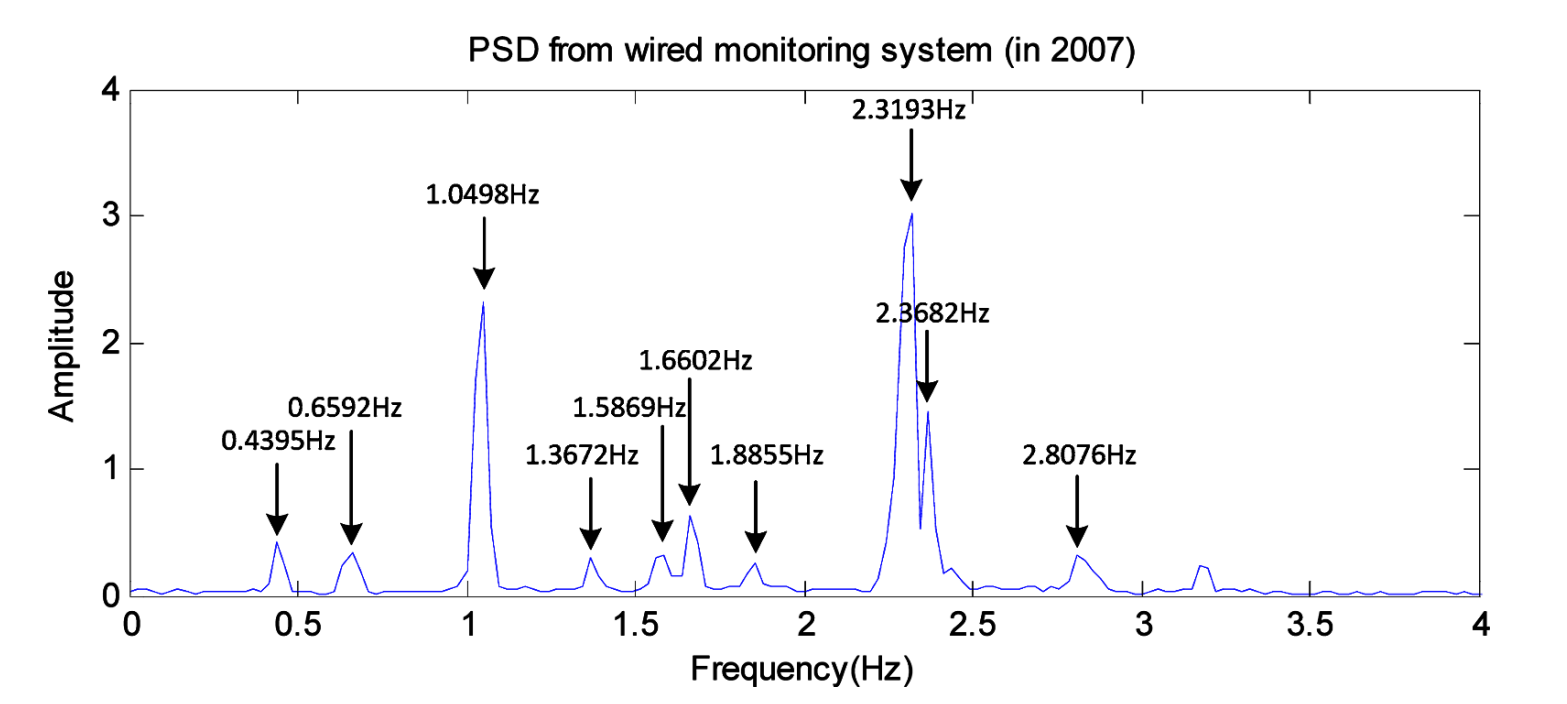
\includegraphics[scale=0.35]{Sections/Literature-Review/bridge-wired-psd.png}
	\label{PSD-Wired}
\end{figure}

The existing literature on LoRaWAN exemplifies the versatility and potential of this technology in various IoT applications, including those demanding long range and low power consumption. Several limitations including the inconsistencies in packet loss, throughput and connectivity, coupled with significant data transmission delay, as outlined in table \ref{Lit-Summary-Table}, present substantial challenges, especially for real-time data analysis and applications requiring consistent downlink messages. Such findings underscore the need for an in-depth understanding of LoRaWAN's performance to address these limitations in this project's system design. 




\begin{table}[!hbt]
\begin{tabular}{|c|l|l|}
\hline
\rowcolor[HTML]{C0C0C0} 
\textbf{Reference}                                               & \multicolumn{1}{c|}{\cellcolor[HTML]{C0C0C0}\textbf{Significant Contribution}}                                                     & \multicolumn{1}{c|}{\cellcolor[HTML]{C0C0C0}\textbf{Limitation}}                                                                                         \\ \hline
\begin{tabular}[c]{@{}c@{}}Gehani et al.\\ (2021)\end{tabular}   & \begin{tabular}[c]{@{}l@{}}LoRa Transmitters can function \\ effectively up to a depth of 50 cm\\ in soil.\end{tabular}            & \begin{tabular}[c]{@{}l@{}}Only 3 m distance between \\ transmitting and receiving \\ node.\end{tabular}                                                 \\ \hline
\begin{tabular}[c]{@{}c@{}}Fox et al.\\ (2019)\end{tabular}      & \begin{tabular}[c]{@{}l@{}}Comprehensive IoT cloud \\ architecture deployment.\end{tabular}                                        & \begin{tabular}[c]{@{}l@{}}Limited transmission\\ capacity and end device \\ battery life.\end{tabular}                                                  \\ \hline
\begin{tabular}[c]{@{}c@{}}Wildan et al. \\ (2020)\end{tabular}  & \begin{tabular}[c]{@{}l@{}}Designed and implemented a GUI \\ for smart home systems leveraging \\ LoRa.\end{tabular}               & \begin{tabular}[c]{@{}l@{}}Data transmission delay \\ averaged 3.86 seconds.\end{tabular}                                                                \\ \hline
\begin{tabular}[c]{@{}c@{}}Maziero et al.\\ (2019)\end{tabular}  & \begin{tabular}[c]{@{}l@{}}Real-time monitoring system for \\ tracking electrical quantities.\end{tabular}                         & \begin{tabular}[c]{@{}l@{}}No explanation for smart \\ meters with packet delivery \\ less than 95\%.\end{tabular}                                       \\ \hline
\begin{tabular}[c]{@{}c@{}}Eridani et al. \\ (2019)\end{tabular} & \begin{tabular}[c]{@{}l@{}}Conducted a series of tests focusing \\ on throughput and packet loss.\end{tabular}                     & \begin{tabular}[c]{@{}l@{}}Inconsistent throughput \\ and significant packet loss.\end{tabular}                                                          \\ \hline
\begin{tabular}[c]{@{}c@{}}Wixted et al. \\ (2016)\end{tabular}  & \begin{tabular}[c]{@{}l@{}}Successful connection and \\ acknowledgement request between \\ an end device and gateway.\end{tabular} & \begin{tabular}[c]{@{}l@{}}Connection was completely \\ lost in isolated stairwells \\ and low with only one gateway.\end{tabular}                       \\ \hline
\begin{tabular}[c]{@{}c@{}}Wang et al. \\ (2019)\end{tabular}    & \begin{tabular}[c]{@{}l@{}}Correlation between packet RSSI \\ and distance was measured.\end{tabular}                              & \begin{tabular}[c]{@{}l@{}}RSSI decreases with distance \\ and is directly influenced by \\ environment, obstacles and \\ spreading factor.\end{tabular} \\ \hline
\begin{tabular}[c]{@{}c@{}}Jang et al. \\ (2010)\end{tabular}    & \begin{tabular}[c]{@{}l@{}}Large scale deployment of WSSNs \\ and two base stations on the Jindo\\ Bridge.\end{tabular}            & \begin{tabular}[c]{@{}l@{}}Linear relationship between \\ number of requested data \\ points and communication time.\end{tabular}                        \\ \hline
\begin{tabular}[c]{@{}c@{}}Cho et al. \\ (2020)\end{tabular}     & \begin{tabular}[c]{@{}l@{}}Analysed data collected from the\\ WSSNs.\end{tabular}                                                  & \begin{tabular}[c]{@{}l@{}}Independent WSSN analysis \\ required due to no \\ synchronization.\end{tabular}                                              \\ \hline
\end{tabular}
\caption{Summary of Reviewed Literature}
\label{Lit-Summary-Table}
\end{table}

In the context of SHM, LoRaWAN presents a compelling alternative to traditional WSNs, such as Wi-Fi, Bluetooth and Zigbee, offering superior range and adaptability whilst satisfying low power requirements and the potential for flexible sensor placement. However, the highlighted limitations from the literature must be carefully addressed in the design of this LoRaWAN-based SHM system. This project will seek to tackle the presented challenges by focusing on the design optimization for the Griffith footbridge monitoring system. In particular, the aim is to strike a balance between computational load, power consumption and data transmission delay whilst ensuring robust and reliable system performance. 